\documentclass[tikz,border=10pt]{standalone}
\usepackage{circuitikz}
\usepackage{xcolor}
\usepackage{amsmath}
\usetikzlibrary{arrows, decorations.pathmorphing, shapes.symbols, positioning}

\begin{document}
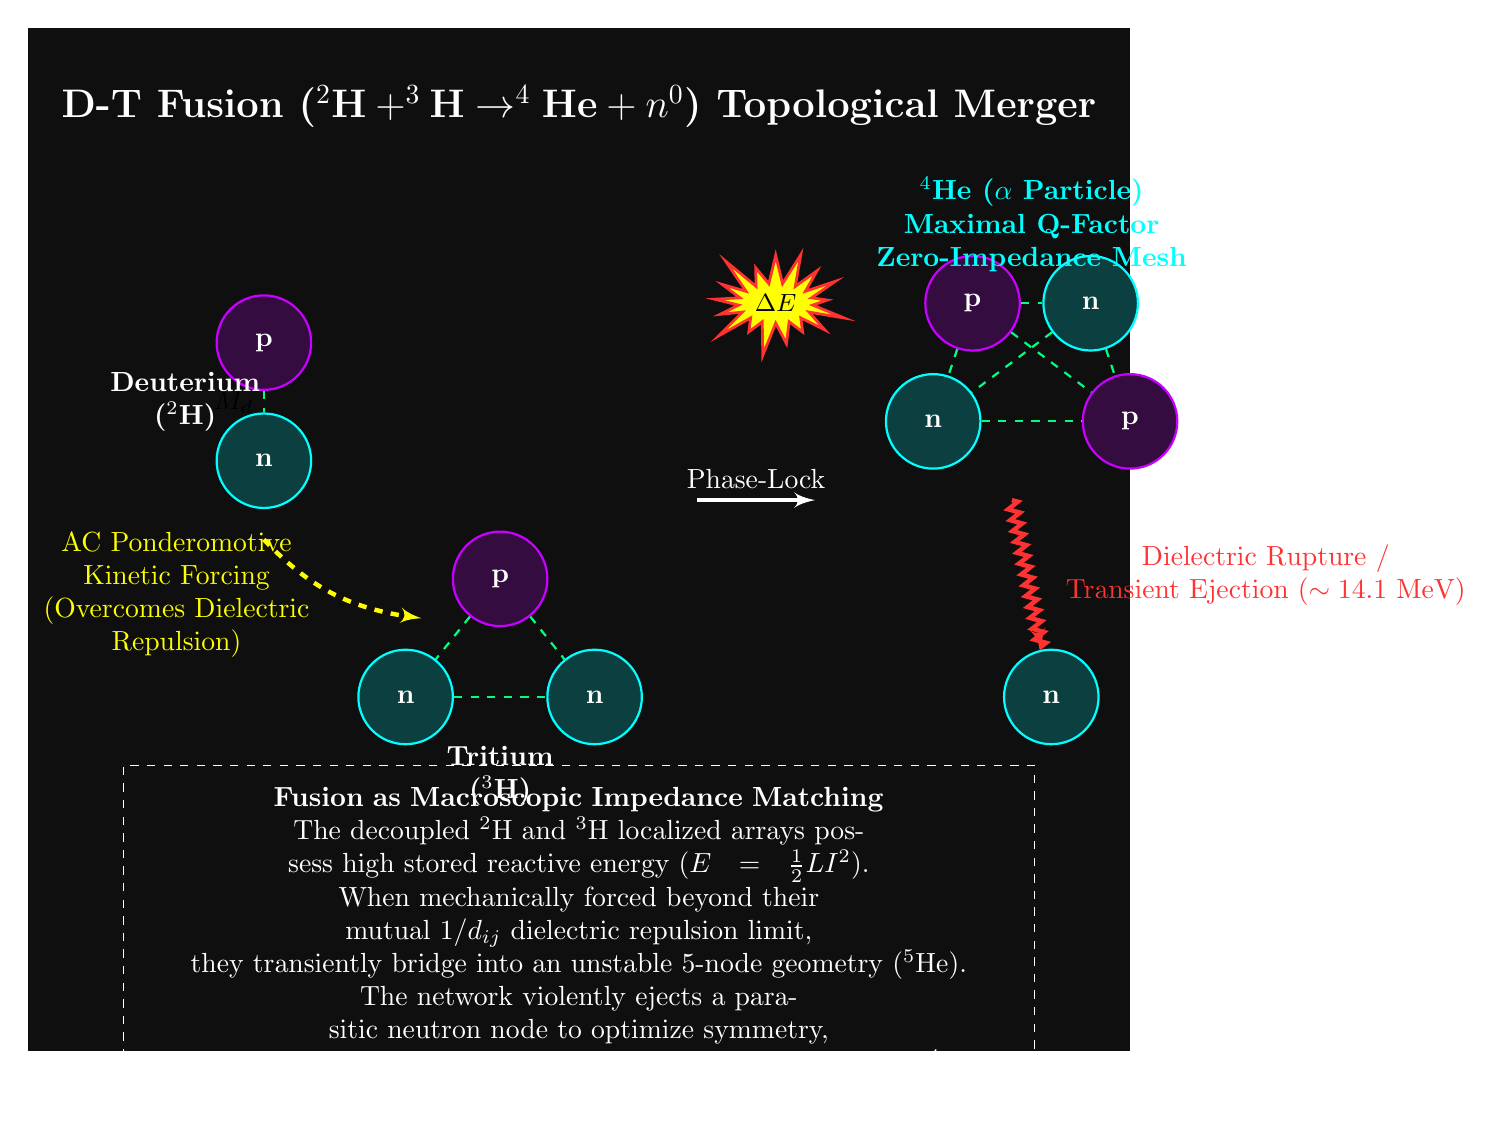
\begin{tikzpicture}[>=latex']

\definecolor{neonblue}{RGB}{0, 255, 255}
\definecolor{neongreen}{RGB}{0, 255, 128}
\definecolor{neonred}{RGB}{255, 50, 50}
\definecolor{neonpurple}{RGB}{200, 0, 255}
\definecolor{darkbg}{RGB}{15, 15, 15}
\definecolor{neonyellow}{RGB}{255, 255, 0}
\definecolor{goldenrod}{RGB}{218, 165, 32}

% Fill background
\fill[darkbg] (-7,-7) rectangle (7,6);

% Title
\node[text=white, font=\bfseries\Large] at (0, 5) {D-T Fusion ($^2\text{H} + ^3\text{H} \rightarrow ^4\text{He} + n^0$) Topological Merger};

\tikzset{
    proton/.style={
        draw=neonpurple, thick, fill=darkbg!80!neonpurple,
        circle, inner sep=2pt, minimum size=1.2cm,
        text=white, font=\bfseries, align=center
    },
    neutron/.style={
        draw=neonblue, thick, fill=darkbg!80!neonblue,
        circle, inner sep=2pt, minimum size=1.2cm,
        text=white, font=\bfseries, align=center
    },
    bus/.style={
        draw=neongreen, thick, dashed
    },
    forced coupling/.style={
        draw=neonyellow, ultra thick, dashed, ->
    },
    ejection/.style={
        draw=neonred, ultra thick, ->, decoration={zigzag, segment length=4pt, amplitude=2pt}, decorate
    }
}

% --- LEFT SIDE: THE INBOUND COLLISION (Unstable State) ---

% Deuterium (2-node linear array)
\node[proton] (Dp) at (-4, 2) {p};
\node[neutron] (Dn) at (-4, 0.5) {n};
\draw[bus] (Dp) -- (Dn) node[midway, left] {$M_{d}$};
\node[text=white, font=\bfseries, align=center] at (-5, 1.25) {Deuterium\\($^2\text{H}$)};

% Tritium (3-node triangular array)
\node[proton] (Tp) at (-1, -1) {p};
\node[neutron] (Tn1) at (-2.2, -2.5) {n};
\node[neutron] (Tn2) at (0.2, -2.5) {n};
\draw[bus] (Tp) -- (Tn1);
\draw[bus] (Tp) -- (Tn2);
\draw[bus] (Tn1) -- (Tn2);
\node[text=white, font=\bfseries, align=center] at (-1, -3.5) {Tritium\\($^3\text{H}$)};

% Kinetic Forcing AC Ponderomotive Drive
\draw[forced coupling] (-4, -0.5) to[bend right=20] node[midway, left=5pt, text=neonyellow, align=center] {AC Ponderomotive\\Kinetic Forcing\\(Overcomes Dielectric\\Repulsion)} (-2, -1.5);

% Transition Arrow
\draw[->, ultra thick, draw=white] (1.5, 0) -- (3, 0) node[midway, above, text=white] {Phase-Lock};

% --- RIGHT SIDE: THE FINAL MERGER (Stable Alpha + Ejection) ---

% Alpha Particle Core (4-node symmetric tetrahedron, drawn 2D)
\node[proton] (Ap1) at (5, 2.5) {p};
\node[neutron] (An1) at (6.5, 2.5) {n};
\node[neutron] (An2) at (4.5, 1) {n};
\node[proton] (Ap2) at (7, 1) {p};

% Alpha internal bus lines (Maximum Q-factor mesh)
\draw[bus] (Ap1) -- (An1); \draw[bus] (Ap1) -- (An2); \draw[bus] (Ap1) -- (Ap2);
\draw[bus] (An1) -- (An2); \draw[bus] (An1) -- (Ap2);
\draw[bus] (An2) -- (Ap2);
\node[text=neonblue, font=\bfseries, align=center] at (5.75, 3.5) {$^4\text{He}$ ($\alpha$ Particle)\\Maximal Q-Factor\\Zero-Impedance Mesh};

% Ejected Neutron
\node[neutron] (EjectedN) at (6, -2.5) {n};
\draw[ejection] (5.5, 0) -- (EjectedN) node[midway, right=10pt, text=neonred, align=center] {Dielectric Rupture /\\Transient Ejection ($\sim 14.1\text{ MeV}$)};

% Energy output tag
\node[starburst, fill=neonyellow, draw=neonred, line width=1pt, inner sep=2pt, font=\bfseries\small, text=black] at (2.5, 2.5) {$\Delta E$};

% Annotations
\node[text=white, text width=11cm, align=center, draw=white, dashed, inner sep=8pt] at (0, -5.5) {
    \textbf{Fusion as Macroscopic Impedance Matching}\\
    The decoupled $^2\text{H}$ and $^3\text{H}$ localized arrays possess high stored reactive energy ($E = \frac{1}{2}LI^2$).\\
    When mechanically forced beyond their mutual $1/d_{ij}$ dielectric repulsion limit,\\
    they transiently bridge into an unstable 5-node geometry ($^5\text{He}$).\\
    The network violently ejects a parasitic neutron node to optimize symmetry,\\
    collapsing into the lowest-impedance Phase-Locked $4\alpha$ lattice ($^4\text{He}$).
};

\end{tikzpicture}
\end{document}
